\documentclass[12pt, letterpaper]{article}

\usepackage{amsmath} % needed for including equations
\usepackage[margin=1in]{geometry} % sets the margins to 1in
\usepackage{graphicx} % needed for figures
\graphicspath{{./figures/}} % allows figures to be placed in a different folder
\usepackage[hang,small,bf]{caption} % sets the style on the figure captions
\usepackage{epstopdf} % converts eps files to pdf to display in the latex document
\usepackage{color}
\newcommand{\red}{\color[rgb]{0.6,0.0,0.0}}
%\usepackage{todonotes}
\newcommand{\todo}[1]{{[\bf \red {TODO: } #1}]}
\usepackage{float}
\usepackage{wrapfig}
\usepackage{tabularx}
\usepackage{color,soul}
\usepackage{pdfpages}

\begin{document}

\begin{titlepage}

\begin{center}

\vspace*{\fill}

\vspace{0.5in}

% Insert your title here
{ \LARGE \bfseries Control Methods for Coordinated, Multi-Arm Manipulation with Soft Robots}\\[.25in]

\large
by\\[.25 in]
% Change your name here
Dustan Kraus\\[1in]

A prospectus submitted to the faculty of\\
Department of Mechanical Engineering\\
Brigham Young University

\vspace{1in}

\today

\vspace*{\fill}

\end{center}

\end{titlepage}

%\thispagestyle{empty}
%
%\begin{center}
%\vspace*{\fill}
%
%\begin{figure}[htbp] %  figure placement: here, top, bottom, or page
%   \centering
%   
\includegraphics[width=2.5in]{byume_logo_clear.jpg} 
%\end{figure}
%
%\vspace{0.5in}
%
%\Large{Prospectus Approval}\\[0.5in]
%
%\end{center}
%
%\hspace*{.47in}
%\begin{minipage}[c]{5.25in}
%
%\normalsize
%
%Prospectus submitted by:
%
%\vspace{.5in}
%
%\makebox[2in]{\hrulefill} \hspace{1in} \makebox[2in]{\hrulefill}
%
%% Change your name here
%\parbox[b]{3in}{Dustan Kraus} \, Date
%\vspace{0.5in}
%
%This prospectus has been approved by each member of the Graduate Committee:
%\vspace{0.5in}
%
%\makebox[2in]{\hrulefill} \hspace{1in} \makebox[2in]{\hrulefill}
%
%\parbox[b]{3in}{Marc Killpack - Chair} \, Date
%\vspace{0.4in}
%
%\makebox[2in]{\hrulefill} \hspace{1in} \makebox[2in]{\hrulefill}
%
%\parbox[b]{3in}{Mark Colton} \, Date
%\vspace{0.4in}
%
%\makebox[2in]{\hrulefill} \hspace{1in} \makebox[2in]{\hrulefill}
%
%\parbox[b]{3in}{Randy Beard} \, Date
%
%\end{minipage}
%
%\vspace*{\fill}
%
%\pagebreak
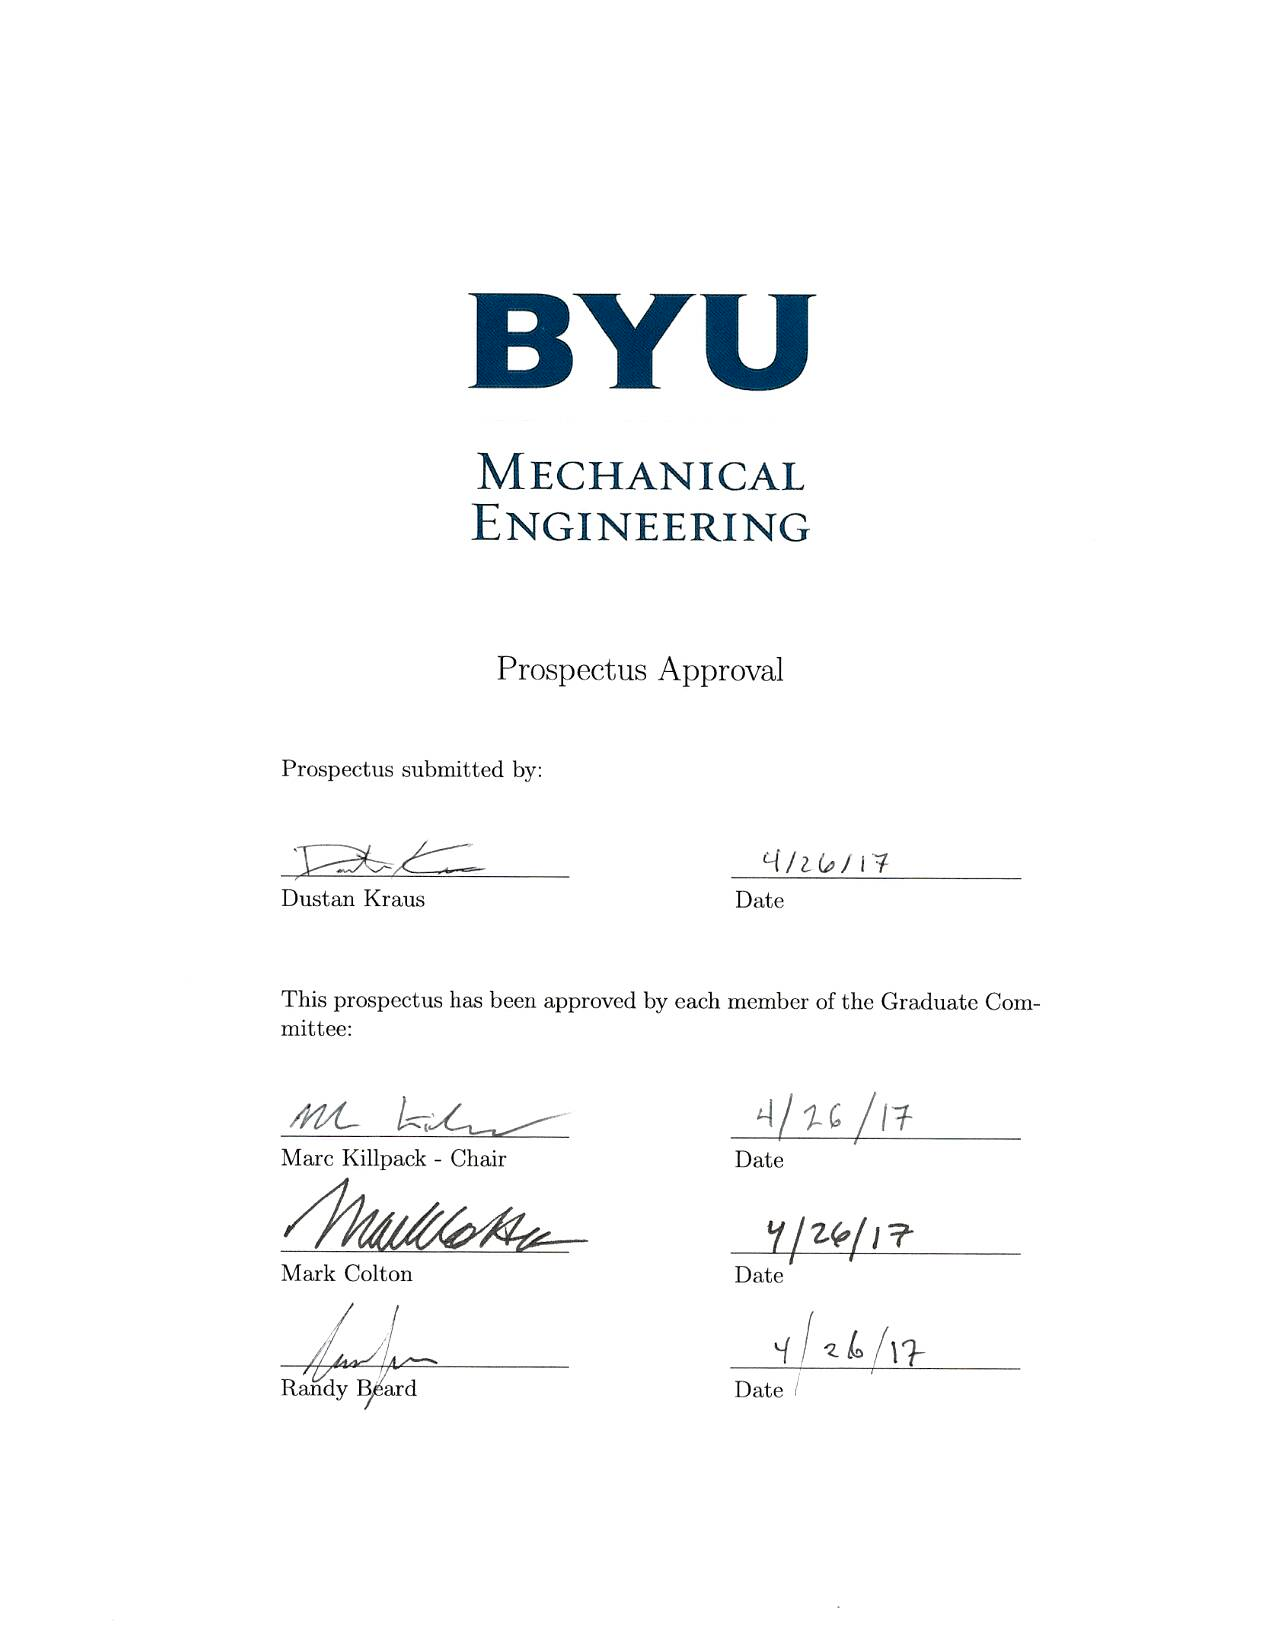
\includepdf[pages={1}]{prospectus_signature_page.pdf}
\setcounter{page}{1}

%%%%%%%%%%%%%%%%%%%%%%%%%%%%%%%%%%%%%%%%%%%%%%%%%%%%%%%%%%%%%%%%%%%%%%%%%%%%%%%%%%%%%%%%%%%%%%%%%%%%%%%
\section{Problem Statement}
% Provide an overview of the problem.
% Finish with an objective statement.
% Address the question: What work is being done?
Every year, the number of robots manufactured increases. Robots play a role in the production of most things we use on a day-to-day basis; however, despite this trend, we have yet to see robots play a more personal role in our daily lives (especially in terms of robot manipulation). 

\begin{wrapfigure}{r}{0.42\textwidth}
  \begin{center}
    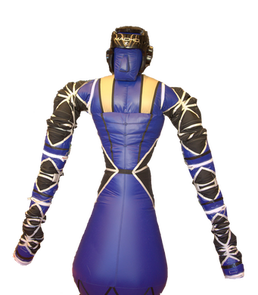
\includegraphics[trim = 0.5cm 0cm 0.5cm 1cm,clip,width=0.3\textwidth]{king_louie.png}
  \end{center}
  \caption{A five degree of freedom soft robot provided by Pneubotics}
  \label{fig:kinglouie}
\end{wrapfigure}

Imagine a robot that could gently help a disabled person into their wheelchair, lift a survivor to safety in a disaster scenario, or even work alongside an astronaut in space. Tasks such as these are difficult, if not impossible, with only one arm. Use of multiple arms makes these types of tasks possible, though traditional robots are not ideally suited for these types of tasks. Industrial robots, though highly precise and capable, have a relatively high inertia and are heavily geared. This severely limits how quickly and safely they can move while operating in close proximity to humans to avoid unexpected collisions and high impact forces.

Development of soft, lightweight robots that are inherently safe around humans will enable robots to play a much more personal role in our lives. My objective is to develop and implement control algorithms for multi-arm manipulation on soft, pneumatically actuated robots (like the one shown in Figure~\ref{fig:kinglouie}). 

\section{Background}
% Briefly review the most relevant literature.
% Provide motivation for the proposed thesis topic.
% Address the questions: What have others done? Why is it important? What are the challenges?
Multi-arm manipulation does not have a specific agreed-upon definition. According to the literature, it could be many fingers on a hand manipulating a small object, or many arms manipulating a large object. In fact, both of these scenarios could use the same control principles. Furthermore, multi-arm manipulation can be categorized by un-coordinated and coordinated tasks. Un-coordinated manipulation tasks are those in which the arms are performing tasks that do not require interaction (e.g., one arm is moving parts while a second arm is performing an unrelated assembly task). Jobs which require two or more robotic arms to physically interact with the same object are classified as coordinated manipulation tasks (see \cite{Smith2012}).  

One difficulty in coordinated, multi-arm manipulation with traditional robots is that small deviations in end effector position or orientation from any of the arms while holding a rigid object can result in large stresses on both the object and internally on the arm. To compensate, many researchers have proposed hybrid force/position control schemes which seek to control the position of an object being grasped by several manipulators while either keeping the forces below a certain threshold or maintaining a certain force (see \cite{Sakaino2011, Alberts1988, Hayati1986, Yoshikawa1993, Uchiyama1988, derventzis1992robust}). Other researchers model the arms connected to the object as a closed kinematic chain, and use a master-slave force control strategy (see \cite{yan2016coordinated}) where the desired trajectory and operational force of the master arm are given in advance and the slave arm's trajectory and operational force are calculated from the closed-chain constraint equations. Other researchers have developed controllers that enforce a controlled impedance of the manipulated object, where the controller compensates for the system dynamics and directly controls the internal forces on the object using force and moment measurements at the robot's wrists (see \cite{schneider1992object, caccavale2008six, erhart2013impedance, ren2016biomimetic}). A challenge with these approaches is the coordination of high bandwidth centralized controllers as any latency can result in dangerously high forces on an object being manipulated. Furthermore, if the software or hardware malfunctions and the force control stops working, traditional robots could exert a dangerous amount of force on the object being manipulated, themselves, humans, or other delicate equipment nearby. Although the occurrence of such an event is low probability, the risk if it does occur is very high. Additionally, transporting traditional heavy robots to many locations where multi-arm manipulation may be useful, such as search and rescue sites, may be expensive or impossible depending on available transportation infrastructure. 

An alternative and novel approach is to mitigate buildup of high forces by using a robot with flexible links and passive compliance in the joints from the compressibility of air. Because soft robots are inherently compliant, deviations in object position result in significantly lower buildup of forces; thus, they lend themselves nicely to tasks involving several arms. Even tasks with one rigid arm and multiple soft arms become simpler as the whole system is forgiving of end effector deviations due to compliance of the soft arms. Therefore, one of the major concerns with successful implementation of coordinated, multi-arm manipulation is eliminated. 

Additionally, because these robots are soft and inherently compliant, they should be inherently safer around humans and delicate equipment even if something malfunctions. They are also much lighter and smaller than traditional robots, and therefore much easier to transport to a disaster scenario for example. On the other hand, compliant links and joints introduce new challenges (addressed below) into the control paradigm, and currently do not perform as well (with regards to metrics like rise time, repeatability, accuracy, and overshoot) as state-of-the-art torque-controlled robots like Robonaut 2. 

Engineers have begun to explore the design and control of soft-bodied robots composed of compliant materials (see \cite{rus2015design} for recent developments in the field of soft robotics). C. Laschi et al. have done work with a multi-arm soft robot to mimic crawling behavior of an octopus (see \cite{li2012octopus, cianchetti2015bioinspired}). Others have done research into soft robot design for different types of locomotion (see \cite{shepherd2011multigait}, \cite{seok2013meshworm}). However, to my knowledge no research on multi-arm manipulation with soft robots has been done. My research will be focused on soft robot, coordinated multi-arm manipulation tasks. 

\section{Research Objectives}
% Briefly list the objectives. The reader should be able to make this list based on the background section.
I propose that coordinated multi-arm manipulation can realistically be implemented with inflatable, pneumatically actuated robots. My goals are to implement general coordinated multi-arm soft robot control that will enable tasks such as accurate manipulation of rigid objects in free space and impact tasks with rigid objects (like sweeping off a solar panel or assembly of construction materials that require impact for insertion). Here are the necessary underlying research questions to address:
\begin{itemize}
\item Two key challenges with soft robots are accuracy and repeatability. The dynamics of the arms can change with a variety of different stimuli such as temperature change, pressure loss through bladder punctures, and actuation hysteresis. Additionally, the bladders often reseat themselves as the arms move. What type of control scheme will result in the highest task space accuracy and repeatability?
\item Which type of control scheme will be most effective in coordinated manipulation tasks for soft robots?
%\item Some tasks require more stiffness than is nominally available in a single soft robot arm. I propose that such tasks could become more feasible by grasping one arm with the other (increasing the rigidity by forming a closed kinematic chain). This type of task would not be feasible with a rigid robot. How will the control scheme need to be altered to accurately control this system?
\end{itemize}
To answer these research questions, there are many intermediate steps described in the following section.

\section{Proposed Research}
% Describe the technical approach.
% Describe the scope of the project and note any delimitations if necessary.
% Describe the equipment and facilities required to complete the project.
% Describe any collaborative efforts.
\textit{Manipulability Improvements}: Recent design changes have left the robot in Figure~\ref{fig:kinglouie} (King Louie) with only four degrees of freedom per arm. To perform general manipulation tasks, each end effector needs to be controllable in at least six degrees of freedom. Furthermore, I recently finished simulating King Louie's reachable workspace (using rigid body joint models to approximate the forward kinematics) and found that  with his current configuration, the volume reachable by both arms is essentially zero (see Figure~\ref{fig:kl_workspace}). While I could still manipulate objects of sufficient size with the current workspace, general multi-arm manipulation tasks are limited by both the object size and the limited dexterity of each arm in the current configuration.

%\begin{figure}[htbp] %  figure placement: here, top, bottom, or page
\begin{wrapfigure}{r}{0.4\textwidth}
   \centering
   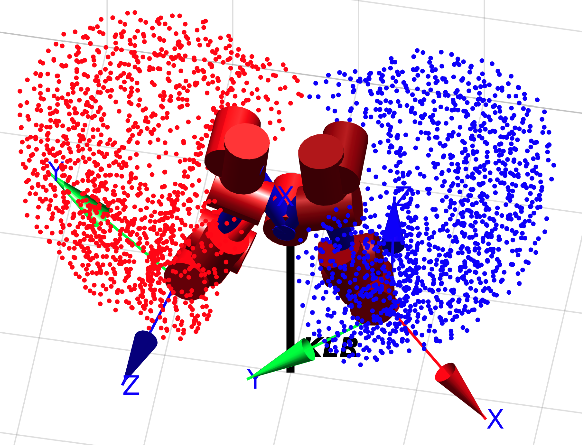
\includegraphics[trim = 0cm 0cm 0cm 0cm,clip,width=2.5in]{KLWorkspace.png}
   \caption{This is a visualization of the current workspace of each of King Louie's arms. The left arm workspace is red, while the right is blue.}
   \label{fig:kl_workspace}
\end{wrapfigure}
%\end{figure}

In order to make general multi-arm manipulation tasks more feasible, I plan on detaching King Louie's arms and remounting them with additional powered degrees of freedom. Another student in my research group recently submitted a paper to ICRA 2017 on rigorous design optimization of soft robots (see \cite{Bodily2017}). I will build on this work in designing an optimization to select which degrees of freedom to add and how to orient the arms to allow for coordinated manipulation tasks. Undergraduate researchers in the lab have designed a way to both mount the arms to a new surface and attach additional degrees of freedom with traditional geared motors. Despite the addition of traditional geared motors, the arms will still be inherently safer around humans than traditional robots because they act as soft, low inertia, low-pass mechanical filters. I will use this mounting technique to implement the results of my optimization, so that I can perform multi-arm manipulation tasks. I hypothesize that the degrees of freedom I add will be at the shoulder and wrist (to allow the end effector to orient itself in any configuration to grasp objects).
	
\textit{Single Arm Hybrid Controller Development}: Task space accuracy and repeatability are affected by dynamic and kinematic modeling error (accurately modeling King Louie and other soft robots is not trivial). Previous researchers in the RaD Lab have designed an algorithm using model predictive control (MPC) that can command a single arm in joint space (see \cite{best2016new}). I have used inverse kinematics libraries – like TRAC-IK (see \cite{beeson2015trac}) in the Robot Operating System to compute desired joint angles for this controller; however, this control method alone does not result in accurate task space positions and orientations due to dynamic and kinematic modeling error. A common control technique to reduce error at the end-effector is visual servoing (see \cite{Wang2016, Vahrenkamp2009}). My first approach to this problem was to create a hybrid controller using an HTC Vive virtual reality system. The Vive uses two IR cameras to report the position and orientation of targets which I used in very preliminary work for servoing feedback to close the end effector position error and improve repeatability. This method is currently very slow, and has some error in the reported end effector position. I plan to tune the controller to get a better response, and optimize the transformations from the vive targets in order to get better accuracy on end effector position.

%This method is currently very slow, and uses the Vive coordinate frames rather than motion capture frames where the robot's DH parameters were defined. I will work on tuning the controller, and optimizing the code to speed it up, and have been working on an optimization to relate the two coordinate frames.  
 
%\begin{figure}[htbp] %  figure placement: here, top, bottom, or page
%   \centering
%   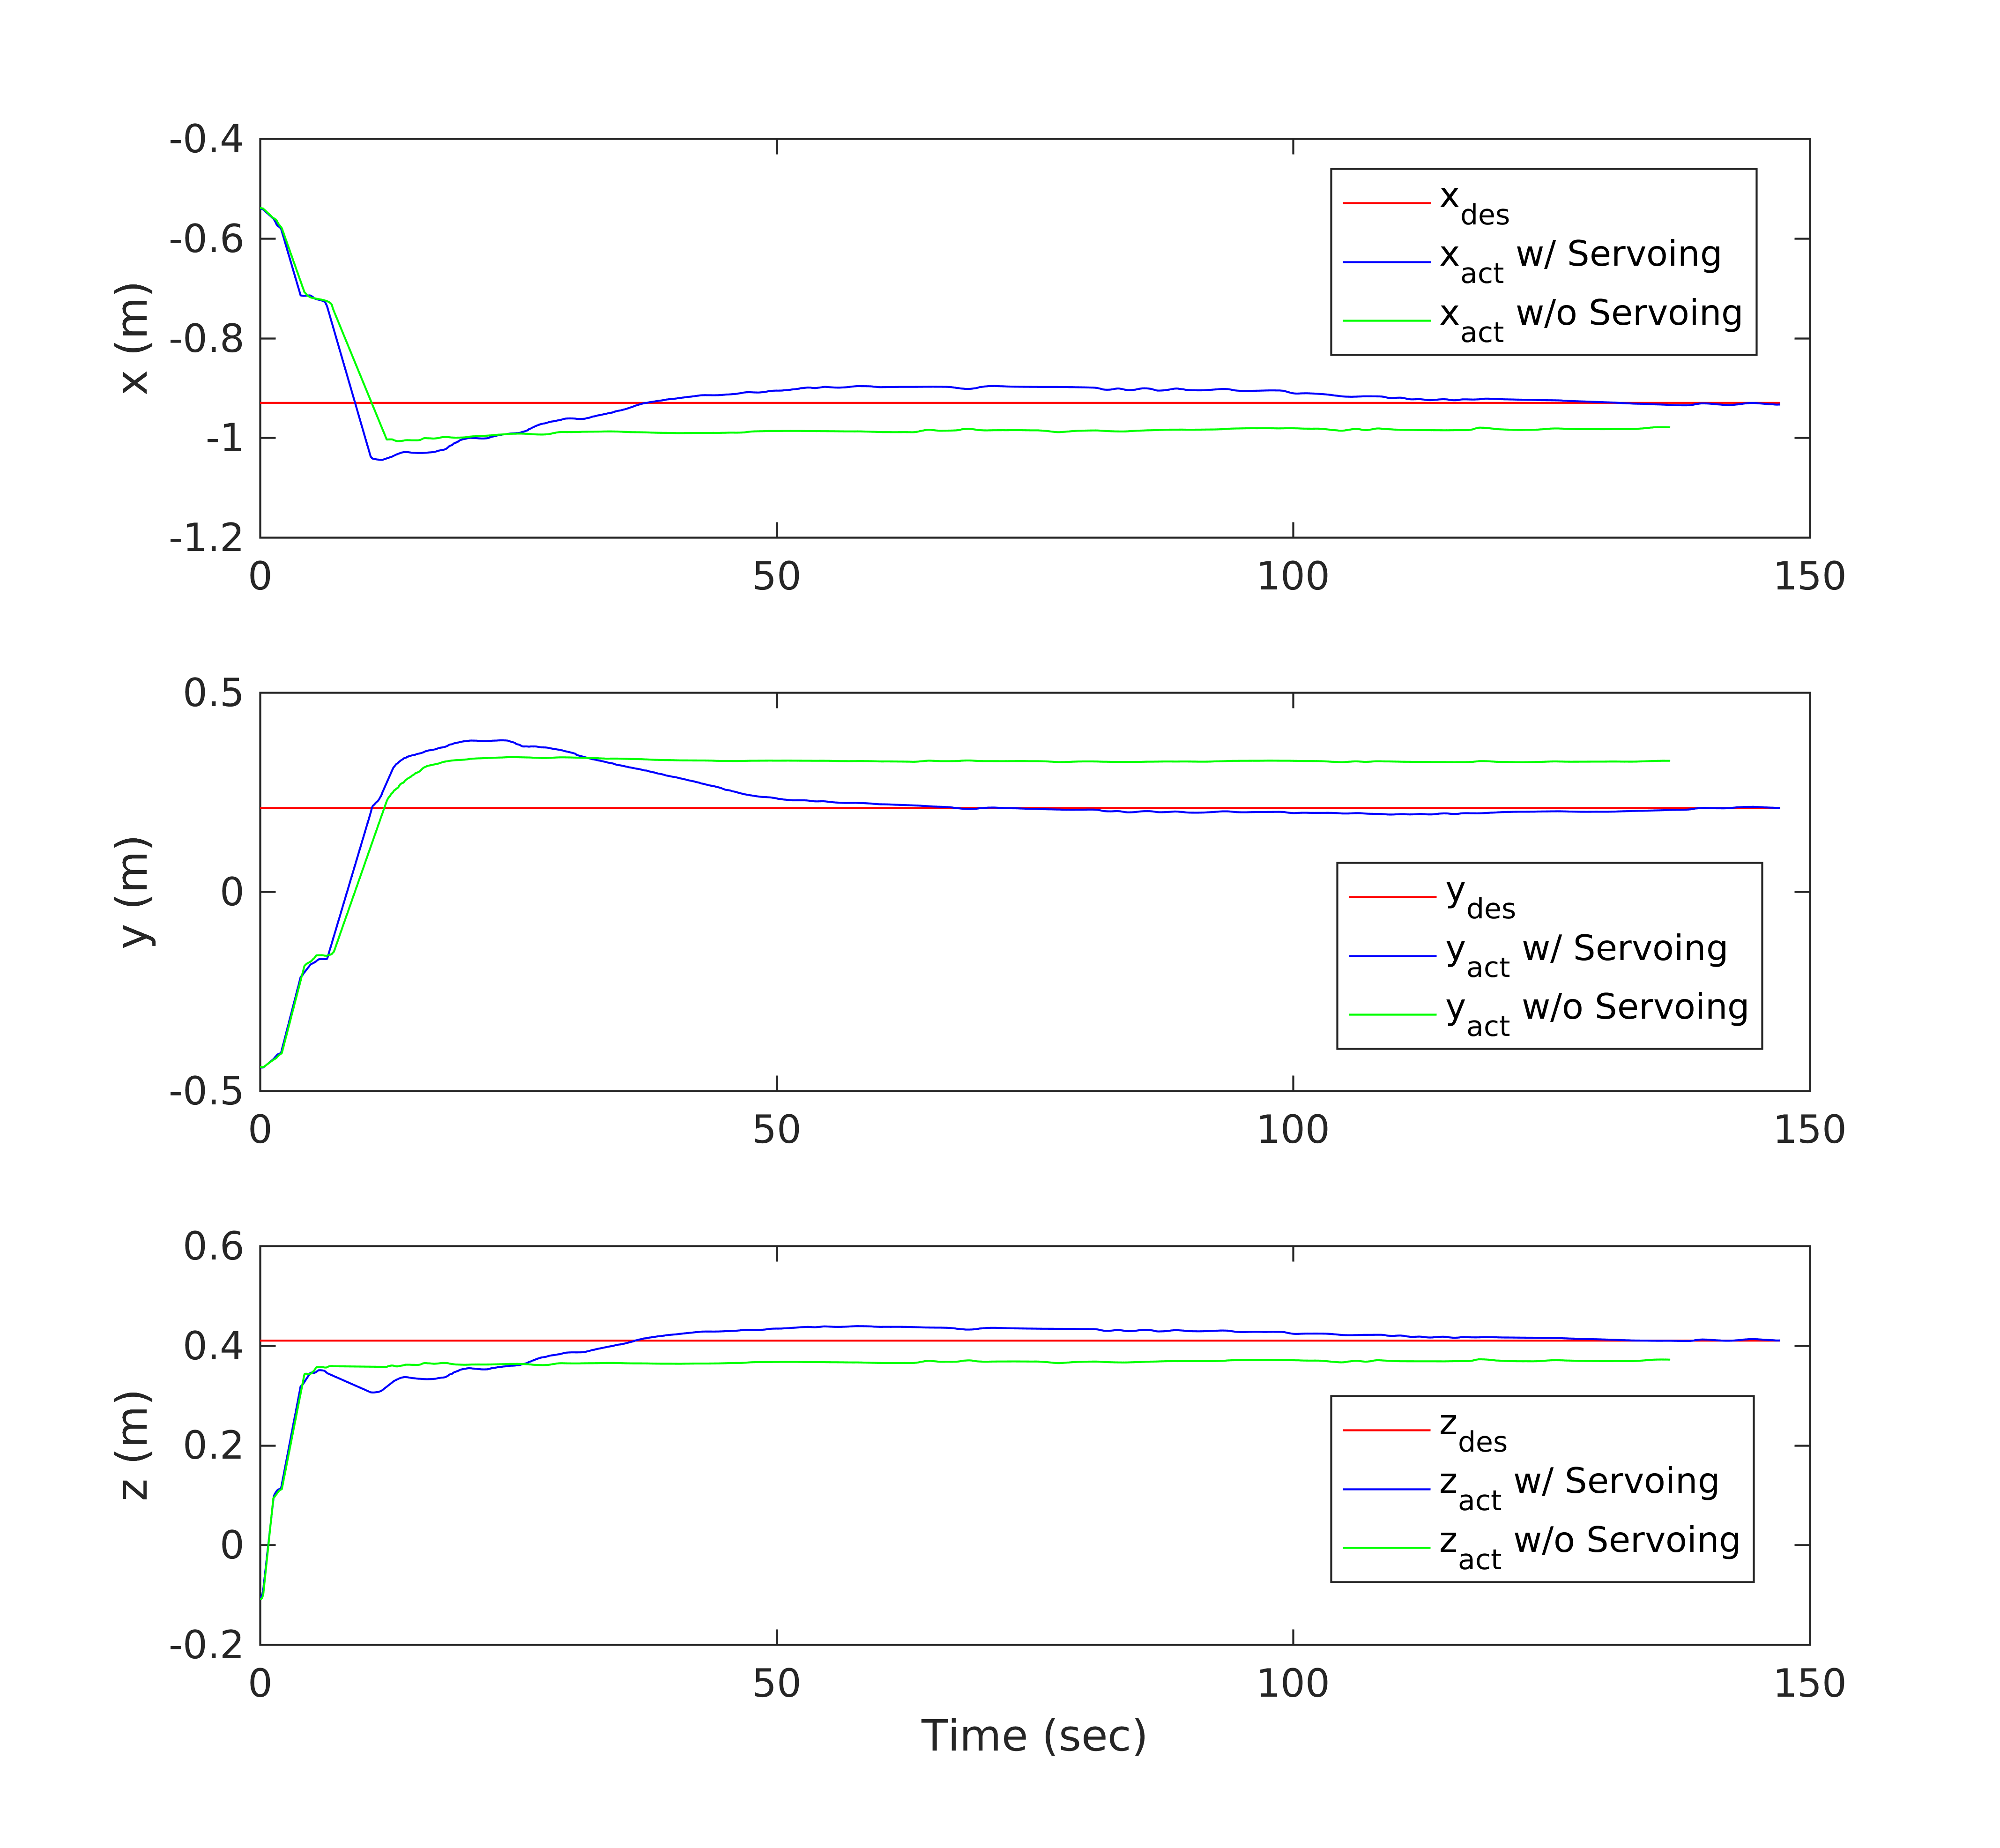
\includegraphics[trim = 0mm 0mm 0mm 0mm,clip,width=6.5in]{servoing.png}
%   \caption{This plot shows that servoing pushes the task space error to zero.}
%   \label{fig:servoing}
%\end{figure}

\textit{Coordinated, Multi-Arm Controller Development}: My first coordinated multi-arm manipulation approach will be to design and implement an object-level model predictive controller. 
\begin{wrapfigure}{r}{0.5\textwidth}
   \centering
   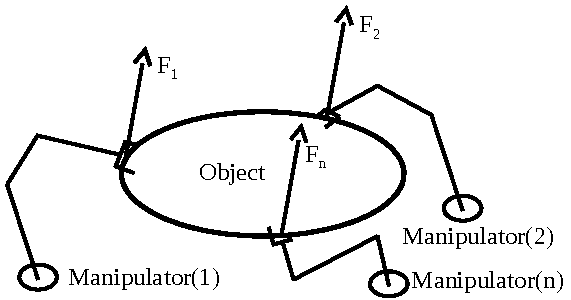
\includegraphics[trim = 0mm 0mm 0mm 0mm,clip,width=3in]{object_level_control_figure.pdf}
   \caption{This shows a figure being manipulated by n robotic manipulators.}
   \label{fig:object_control}
\end{wrapfigure}
MPC uses a system's dynamics to predict the control inputs that will result in desired system motion over a short time horizon. In this case, the system is the object, and there are n robotic manipulators grasping the object in 3D space as shown in Figure~\ref{fig:object_control}. 

The control inputs produced by MPC will be forces and torques to be applied to the object by each manipulator grasping the object. Initially, I will assume that I know the dynamics of the object (by using objects that I can easily calculate the inertia of). These models will likely have error, but previous research with MPC has found it to be robust to modeling error (even with plus or minus half of nominal mass values) (see \cite{killpack2013fast, killpack2013model}). My proposed control scheme is of the form shown in Figure~\ref{fig:control_diagram}. 

\begin{figure}[htbp] %  figure placement: here, top, bottom, or page
   \centering
   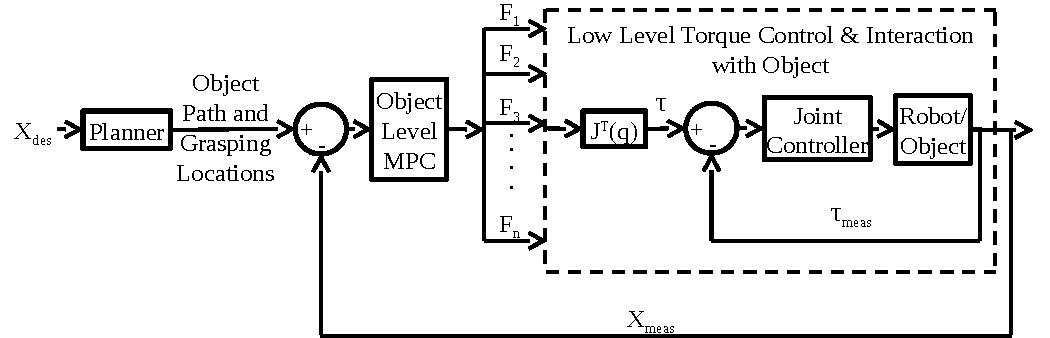
\includegraphics[trim = 0mm 0mm 0mm 0mm,clip,width=6.5in]{control_block_diagram_smaller.pdf}
   \caption{This figure shows the proposed object level MPC control scheme.}
   \label{fig:control_diagram}
\end{figure}

$X_{des}$ and $X_{meas}$ are desired and measured end effector position and orientation, $F_1$ to $F_n$ are wrenches at the end effector of each arm which are fed into a low level joint torque controller, and J is the Jacobian of each arm. Part of answering my research questions above is how to get the soft robots to exert the proper wrench and displacement at the end effector. I will design this controller to be very modular. The first module to develop will be the Object Level MPC block. I have already derived the dynamic equations for an object in 3D space with n forces and torques applied to the object. This module will calculate the desired wrenches to be applied to the object given a desired and current location/trajectory as well as the object dynamics. The next module will be the robotic manipulator control. To design this module, I will need to figure out the best control scheme to achieve the desired wrenches at the end of each manipulator. The final module is the planning module. The long term goal of this module is twofold. First, the module will need to compute optimal grasping locations for each end effector. I hypothesize that these locations will be determined by the robot kinematics as well as the weight distribution and desired configuration of the object. Second, given grasping locations for each end effector, the module will need to compute a desired trajectory for each end effector. This path must be constrained to object motion that is possible given the force/torque and kinematic constraints of the robot manipulators. The second part of the planning module is outside the scope of my proposed thesis, and I will only work on it at a minimal level. My focus for the planning module will be where to grab the object.

Once I can accurately and repeatably manipulate objects using the two arms on the robot in Figure ~\ref{fig:kinglouie}, I will expand my research to utilize more soft arms. This will demonstrate the applicability of my algorithms to systems that include more than two arms.

\section{Anticipated Contributions and Timeline}
% Describe any publications, (including publication venues) patents, or other scholarly products that are anticipated to result from the proposed project.
My anticipated timetable for research progress and publications is included below in table~\ref{tab:publications}.

\noindent
\begin{table}[H]
\centering
\begin{tabularx}{0.99\textwidth}{|X|X|}%{ |m{4cm}|m{3cm}|}
%\begin{tabu} to 0.99\textwidth { | X[lm] | X[rm] | }
 \hline
 Co-submit work on servoing and coordinate frame transformation optimization to robotics journal & \multicolumn{1}{|r|}{May 2017} \\%[3em]
 \hline
 Submit conference paper on object level mpc with two arms given grasping locations, object model, and desired object path to the International Conference on Robotics and Automation 2018 (ICRA 2018). At this point the planning module will not have been developed. & \multicolumn{1}{|r|}{September 2017} \\%[3em]
 \hline
 Submit to robotics journals on initial implementation of full system (planning module, as well as object level mpc)  & \multicolumn{1}{|r|}{April 2018} \\%[1em]
 \hline
\end{tabularx}
\caption{This table contains the anticipated publications that will result from my proposed project.}
\label{tab:publications}
\end{table}

In summary, I expect to have developed and implemented a method for multi-arm manipulation on soft, pneumatically actuated robots. This will be a step forward in developing soft robots that play a much more personal role in our lives.

\pagebreak

\bibliographystyle{IEEEtran}
\bibliography{library}

\end{document}